%!TEX root = ../Thesis.tex
%% Basierend auf TeXnicCenter-Vorlage von Mark Müller
%%                      Willi Nüßer
%%                      Waldemar Penner     
%%                      Ulrich Reus
%%                      Frank Plass
%%                      Oliver Tribeß 
%%                      Daniel Hintze     
%%%%%%%%%%%%%%%%%%%%%%%%%%%%%%%%%%%%%%%%%%%%%%%%%%%%%%%%%%%%%%%%%%%%%%%

% Wählen Sie die Optionen aus, indem Sie % vor der Option entfernen  
% Dokumentation des KOMA-Script-Packets: scrguide

%%%%%%%%%%%%%%%%%%%%%%%%%%%%%%%%%%%%%%%%%%%%%%%%%%%%%%%%%%%%%%%%%%%%%%%
%% Optionen zum Layout des Artikels (Xetex informieren. Ist schön)   %%
%%%%%%%%%%%%%%%%%%%%%%%%%%%%%%%%%%%%%%%%%%%%%%%%%%%%%%%%%%%%%%%%%%%%%%%
\documentclass[%
paper=A4,         % alle weiteren Papierformat einstellbar
fontsize=12pt,    % Schriftgröße (12pt, 11pt (Standard))
BCOR12mm,         % Bindekorrektur, bspw. 1 cm
DIV14,            % breiter Satzspiegel
parskip=half*,    % Absatzformatierung s. scrguide 3.1
headsepline,      % Trennline zum Seitenkopf  
%footsepline,     % Trennline zum Seitenfuß
%normalheadings,  % Überschriften etwas kleiner (smallheadings)
listof=totoc,     % Tabellen & Abbildungsverzeichnis ins Inhaltsverzeichnis      
%bibtotoc,        % Literaturverzeichnis im Inhalt 
%draft            % Überlangen Zeilen in Ausgabe gekennzeichnet
footinclude=false,% Fußzeile in die Satzspiegelberechnung einbeziehen 
headinclude=true, % Kopfzeile in die Satzspiegelberechnung einbeziehen 
oneside,          % laut Internet nur eine Seite Inhaltsverzeichnis
final             % draft beschleunigt die Kompilierung final ist standard
]
{scrartcl}

%\setuptoc{toc}{totoc} % Inhaltsverzeichnis ins Inhaltsverzeichnis

% Neue Deutsche Rechtschreibung und Deutsche Standardtexte
\usepackage[ngerman]{babel} 

% Umlaute können verwendet werden
\usepackage[utf8]{inputenc}   

% Echte Umlaute
\usepackage[T1]{fontenc} 

% Latin Modern Font, Type1-Schriftart für nicht-englische Texte
\usepackage{lmodern} 

% 1/2-zeiliger Zeilenabstand
\usepackage[onehalfspacing]{setspace}

% Für die Defenition eigener Kopf- und Fußzeilen
\usepackage{fancyhdr} 

% Für die Verwendung von Grafiken
\usepackage[pdftex]{graphicx} %( [...,draft] verhindert Bilder Kompilieren)

% Bessere Tabellen
\usepackage{tabularx}

% Für die Befehle \toprule, \midrule und \bottomrule, z.B. in Tabellen 
\usepackage{booktabs}

% Erlaubt die Benutzung von Farben
\usepackage{color}
\usepackage{colortbl}

% Links im PDF
\usepackage{hyperref}

% Verbessertes URL-Handling mit \url{http://...}
\usepackage{url}

% Listen ohne Abstände \begin{compactlist}...\end{compactlist}
\usepackage{paralist} 

% Ausgabe der aktuellen Uhrzeit für die Draft-Versionen
\usepackage{datetime}

% Deutsche Anführungszeichen
\usepackage[babel,german=quotes]{csquotes}

% Verbessert das Referenzieren von Kapiteln, Abbildungen etc.
\usepackage[german,capitalise]{cleveref}

% Konfiguration der Abbildungs- und Tabellenbezeichnungen
% \usepackage[format=hang, font={footnotesize, sf}, labelfont=bf, justification=raggedright,singlelinecheck=false]{caption}
\usepackage[format=hang, font={footnotesize, sf}, labelfont=bf, justification=justified,singlelinecheck=false]{caption}

% Verbessert die Lesbarkeit durch Mikrotypografie
\usepackage[activate={true,nocompatibility},final,tracking=true,kerning=true,spacing=true,factor=1100,stretch=10,shrink=10]{microtype} 

% Zitate und Quellenverzeichnis der Vorlage
\usepackage[
    style=authoryear,         % Zitierstil
    firstinits=false,         % false = Vornamen werden ausgeschrieben
    natbib=true,
    urldate=long,             % "besucht am" - Datum
    %url=false,
    date=long,                
    dashed=false, 
    maxcitenames=3,           % max. Anzahl Autorennamen in Zitaten
    maxbibnames=99,           % max. Anzahl Autorennamen im Quellenverzeichnis
    %backend=bibtex           % Ggf. für ältere Distributionen bibtex verwenden
    backend=biber
]{biblatex}
\DeclareNameAlias{sortname}{first-last}

% Bibliograpthy
\bibliography{library/library}

% Keine Einrückung bei einem neuen Absatz 
\parindent 0pt 

% Ebenentiefe der Nummerierung
\setcounter{secnumdepth}{3}

% Gliederungstiefe im Inhaltsverzeichnis 
\setcounter{tocdepth}{3} 

% Tabellen- und Abbildungsverzeichnis mit Bezeichnung:
\usepackage[titles]{tocloft}

% Sourcecode-Listings
\usepackage{listings}
% Bestimmte Warnungen unterdrücken
% siehe http://tex.stackexchange.com/questions/51867/koma-warning-about-toc
\usepackage{scrhack} 

%%%%%%%%%%%%%%%%%%%%%%%%%%%%%%%%%%%%%%%%%%%%%
% Von An-Nam benötigte packages
%%%%%%%%%%%%%%%%%%%%%%%%%%%%%%%%%%%%%%%%%%%%%

% Für Pfeile in Textmodus
\usepackage{textcomp}

% Für farbige Umrandungen bei Texten
\usepackage{tcolorbox}

% Für Definitionen in ausgegrauten Kästchen
\usepackage{thmbox}
\usepackage{shadethm}

%Zum Durchstreichen und weiterer Textformatierungen
\usepackage{ulem}

% Mehr Funktionen bei Rahmen und Boxen
\usepackage[]{mdframed}

% Mehrseitige PDFs einbinden
\usepackage{pdfpages}

% Um Bildbeschriftungen von mehreren Bildern nebeneinander anzuzeigen
%\usepackage{subfig}
\usepackage{subcaption}

% Um Bilder an der Seite und Text daneben
\usepackage{wrapfig}

% Sidecap für Textbeschriftung neben Bild
\usepackage{sidecap}

% Große Math Symbole
\usepackage{relsize}

%Für mehr Mathe
\usepackage{amsmath}
\usepackage{amssymb}

% Float
\usepackage{float}

% Pifont und Marvosymfür Aufzählungszeichen
\usepackage{pifont}
\usepackage{marvosym}
%Initialen (großer Erstbuchstabe)
\usepackage{lettrine}

% Verhindert Silbentrennung
%\usepackage[none]{hyphenat}

% Silbentrennung an Wortfuge
% \usepackage{hyphsubst} 

% Mehr als ein optionaler Parameter in neuen Befehlen
\usepackage{xargs}

% Farbiger Text
\usepackage[pdftex,dvipsnames]{xcolor}

%Tikz für Graphiken
\usepackage{tikz}

% Für Abbildungsnummering nach Kapiteln
\usepackage{chngcntr}
\counterwithin{figure}{section}

% Visio Import
\usepackage{epsfig}
\usepackage{mathtools}
\usepackage{transparent}

% Todo Notizen
\usepackage[colorinlistoftodos,prependcaption,textsize=tiny]{todonotes}

% http://tex.stackexchange.com/questions/126839/how-to-add-a-colon-after-listing-label


\makeatletter
\begingroup\let\newcounter\@gobble\let\setcounter\@gobbletwo
  \globaldefs\@ne \let\c@loldepth\@ne
  \newlistof{listings}{lol}{\lstlistlistingname}
\endgroup
\let\l@lstlisting\l@listings
\makeatother

% Bilder nicht kompilieren
% \renewcommand*\includegraphics[2][]{}

\renewcommand*\cftfigpresnum{Abbildung~}
\renewcommand*\cfttabpresnum{Tabelle~}
\renewcommand*\cftlistingspresnum{Listing~}
\renewcommand{\cftfigaftersnum}{:~~}
\renewcommand{\cfttabaftersnum}{:}
\renewcommand{\cftlistingsaftersnum}{:}
\settowidth{\cftfignumwidth}{\cftfigpresnum 99~\cftfigaftersnum}
\settowidth{\cfttabnumwidth}{\cfttabpresnum 99~\cftfigaftersnum}
\settowidth{\cftlistingsnumwidth}{\cftlistingspresnum 99~\cftfigaftersnum}
\setlength{\cfttabindent}{1.5em}
\setlength{\cftfigindent}{1.5em}
\setlength{\cftlistingsindent}{1.5em}

\renewcommand\lstlistlistingname{Listingverzeichnis}
 
% Style für Kopf- und Fußzeilenfelder
\pagestyle{fancy}
\fancyhf{}
\fancyhead[R]{\leftmark}
\fancyfoot[R]{\thepage} 
\renewcommand{\sectionmark}[1]{\markboth{#1}{#1}} 
\fancypagestyle{plain}{}

% Macro für Quellenangaben unter Abbildungen und Tabellen (Original)
% \newcommand{\source}[1]{{\vspace{-1mm}\\\footnotesize\textsf{\textbf{Quelle:}} \textsf{#1}\par}}

% Macro für Quellenangaben unter Abbildungen und Tabellen (Für An-Nam)
\newcommand{\source}[1]{{\vspace{-1mm}\footnotesize\textsf{\textbf{Quelle:}} \textsf{#1}\par}}
% Anpassungen der Formatierung an Eclipse-Aussehen 
% http://jevopi.blogspot.de/2010/03/nicely-formatted-listings-in-latex-with.html
%\definecolor{sh_comment}{rgb}{0.12, 0.38, 0.18 } %adjusted, in Eclipse: {0.25, 0.42, 0.30 } = #3F6A4D
%\definecolor{sh_keyword}{rgb}{0.37, 0.08, 0.25}  % #5F1441
%\definecolor{sh_string}{rgb}{0.06, 0.10, 0.98} % #101AF9
% Für Druckausgabe sollte alles schwarz sein
\definecolor{sh_comment}{rgb}{0.0, 0.0, 0.0 }
\definecolor{sh_keyword}{rgb}{0.0, 0.0, 0.0 }
\definecolor{sh_string}{rgb}{0.0, 0.0, 0.0 }

\lstset{ %
  language=Java,
  basicstyle=\footnotesize\ttfamily,
  fontadjust, 
  xrightmargin=1mm,
  xleftmargin=5mm,
  tabsize=2,
  columns=flexible,
  showstringspaces=false,
  rulesepcolor=\color{black},
  showspaces=false,showtabs=false,tabsize=2,
  stringstyle=\color{sh_string},
  keywordstyle=\color{sh_keyword}\bfseries,
  commentstyle=\color{sh_comment}\itshape,
  captionpos=t,
  lineskip=-0.3em
}

%\makeatletter
%\def\l@lstlisting#1#2{\@dottedtocline{1}{0em}{1.5em}{\lstlistingname\space{#1}}{#2}}
%\makeatother

% Anhangsverzeichnis
\usepackage[nohints]{minitoc} %Anhangsverzeichnis

\makeatletter
\newcounter{fktnr}\setcounter{fktnr}{0}
\newcounter{subfktnr}[fktnr]\setcounter{subfktnr}{0}

\renewcommand\thesubfktnr{\arabic{fktnr}.\arabic{subfktnr}}
\newcounter{anhangcounter}
\newcommand{\blatt}{\stepcounter{anhangcounter}}

\newcommand{\anhang}[1]{\setcounter{anhangcounter}{0}\refstepcounter{fktnr}
\addcontentsline{fk}{subsection}{Anhang~\thefktnr: \hspace*{1em}#1}
\subsection*{{Anhang~\thefktnr \hspace*{1em} #1 \hspace*{-1em}}}
}

\newcommand{\subanhang}[1]{\setcounter{anhangcounter}{0}\refstepcounter{subfktnr}
\addcontentsline{fk}{subsubsection}{Anhang~\thesubfktnr: \hspace*{1em}#1}
\subsubsection*{{Anhang~\thesubfktnr \hspace*{1em} #1 \hspace*{-1em}}}
}

\newcommand{\anhangsverzeichnis}{\mtcaddsection{\subsection*{Anhangsverzeichnis \@mkboth{FKT}{FKT}}}\@starttoc{fk}\newpage}

% Abkürzungsverzeichnis
\usepackage[acronym,         % create list of acronyms
            nonumberlist,
            toc, 
            section,
            nomain,          % don't need main glossary for this example
            hyperfirst=false,% don't hyperlink first use
            sanitize=none    % switch off sanitization as description
            ]{glossaries}
            \newglossarystyle{mylist}{%
\setglossarystyle{long}% base this style on the list style
\renewcommand*{\glossaryentryfield}[5]{%
    \glsentryitem{##1}\textbf{##2} & ##3 \\}%
}


% \newacronym{Verweislabel}{Abkürzung}{Lang ausgeschrieben}

\newacronym{FTP}{FTP}{File Transfer Protocol}
\newacronym{IaaS}{IaaS}{Infrastructure as a Service}
\newacronym{ITIL}{ITIL}{IT Infrastructure Library}
\newacronym{SLA}{SLA}{Service Level Agreement}
\newacronym{ERP}{ERP}{Enterprise-Resource-Planning}
\newacronym{CRM}{CRM}{Customer-Relationship-Management}
\newacronym{RDS}{RDS}{Rapid Deployment Solution}
\newacronym{ITBA}{ITBA}{IT-Business-Alignment}
\setglossarystyle{mylist}
%\makeglossaries\myglossaries
\makeglossaries

%%%%%%%%%%%%%%%%%%%%%%%%%%%%%%%%%%%%%%%%%%%%%%%%%%%%%%%%%%%%%%%%%%%%%%%
%% Parameter - Hier auf die eigene Arbeit anpassen
%%%%%%%%%%%%%%%%%%%%%%%%%%%%%%%%%%%%%%%%%%%%%%%%%%%%%%%%%%%%%%%%%%%%%%%

\newcommand{\dokumententyp}{Schriftliche Ausarbeitung}
% \newcommand{\abgabedatum}{\today} 
\newcommand{\abgabedatum}{22. April 2016} 
\newcommand{\ort}{Bergisch Gladbach} 
\newcommand{\koorperationsunternehmen}{ComSol AG}
\newcommand{\dokumententitel}{Optimierung der IT für das Startup Stylez}
\newcommand{\dokumentenautor}{An-Nam Pham}
\newcommand{\dokumentenautoradress}{Koppelsweg 23\\50127 Bergheim}
\newcommand{\dokumentenautornummer}{Matrikelnummer: 2316600}
\newcommand{\dokumentenpruefer}{Benno Klaas}

\newcommandx{\technischnotiz}[2][1=]{\todo[linecolor=red,backgroundcolor=red!25,bordercolor=red,#1]{#2}}
\newcommandx{\inhaltnotiz}[2][1=]{\todo[linecolor=blue,backgroundcolor=blue!25,bordercolor=blue,#1]{#2}}
\newcommandx{\verbesserungnotiz}[2][1=]{\todo[linecolor=OliveGreen,backgroundcolor=OliveGreen!25,bordercolor=OliveGreen,#1]{#2}}

\newcommandx{\technischnotizzeile}[2][1=]{\todo[inline,linecolor=red,backgroundcolor=red!25,bordercolor=red,#1]{#2}}
\newcommandx{\inhaltnotizzeile}[2][1=]{\todo[inline,linecolor=blue,backgroundcolor=blue!25,bordercolor=blue,#1]{#2}}
\newcommandx{\verbesserungnotizzeile}[2][1=]{\todo[inline,linecolor=OliveGreen,backgroundcolor=OliveGreen!25,bordercolor=OliveGreen,#1]{#2}}

% \newcommandx{\improvement}[2][1=]{\todo[linecolor=Plum,backgroundcolor=Plum!25,bordercolor=Plum,#1]{#2}}
% \newcommandx{\thiswillnotshow}[2][1=]{\todo[disable,#1]{#2}}

% Infos zu Notizbefehlen:
% http://tex.stackexchange.com/questions/9796/how-to-add-todo-notes
%%%%%%%%%%%%%%%%%%%%%%%%%%%%%%%%%%%%%%%%%%%%%%%%%%%%%%%%%%%%%%%%%%%%%%%

\hypersetup{
  colorlinks=false,
  pdfborder={0 0 0},
  pdftitle=\dokumententitel,
  pdfauthor=\dokumentenautor
} 

\begin{document}

%%%%%%%%%%%%%%%%%%%%%%%%%%%%%%%%%%%%%%%%%%%%%%%%%%%%%%%%%%%%%%%%%%%%%%%
%% Titelseite
%%%%%%%%%%%%%%%%%%%%%%%%%%%%%%%%%%%%%%%%%%%%%%%%%%%%%%%%%%%%%%%%%%%%%%%

%!TEX root = ../Thesis.tex
\begin{titlepage}
\begin{center}


\includegraphics[scale=1.20]{img/fhdw.pdf}\\
\vspace{2cm}
\Huge{\bfseries\dokumententyp}
~\vspace{.5cm}\\
\LARGE{\dokumententitel}
~\vspace{2cm}\\

\large{

\textbf{Prüfer:}\vspace{1mm}\\
\dokumentenpruefer

\vspace{1.5cm}

\textbf{Verfasser:}\\\vspace{1mm}
\dokumentenautor\\
\dokumentenautoradress\\
\dokumentenautornummer
% An-Nam Pham (Mat.Nr.: 2316600)\\
% Koppelsweg 23, 50127 Bergheim\\
% \vspace{5mm}
% Leonie Schiburr (Mat.Nr.: 2316358)\\
% Ferdinand-Schäfer-Straße 8, 51519 Odenthal\\
% \vspace{5mm}
% Vasilij Schneidermann (Mat.Nr.: 2316292)\\
% Rosmarstraße 7, 50226 Frechen

\vspace{1cm}
Studiengang: Wirtschaftsinformatik\\
Spezialisierungsbereich: IT-Consulting

\vspace{0.75cm}
\textbf{Eingereicht am:}\vspace{1mm}\\
\abgabedatum
}
\end{center}

\end{titlepage}


%%%%%%%%%%%%%%%%%%%%%%%%%%%%%%%%%%%%%%%%%%%%%%%%%%%%%%%%%%%%%%%%%%%%%%%
%% Draft-Einstellungen
%%
%% Für die finale Version auskommentieren!
%%%%%%%%%%%%%%%%%%%%%%%%%%%%%%%%%%%%%%%%%%%%%%%%%%%%%%%%%%%%%%%%%%%%%%%
%\fancyhead[L]{\color{red} Stand: \today~-~\currenttime}

%%%%%%%%%%%%%%%%%%%%%%%%%%%%%%%%%%%%%%%%%%%%%%%%%%%%%%%%%%%%%%%%%%%%%%%
%% Verzeichnisse Inhalt
%%%%%%%%%%%%%%%%%%%%%%%%%%%%%%%%%%%%%%%%%%%%%%%%%%%%%%%%%%%%%%%%%%%%%%%

% Römische Seitennummerierung
\pagenumbering{Roman}

% Hinweise und Notizen
% \include{Kapiteln/Hinweise}
% \include{Kapiteln/Notizen}

% Sperrvermerk und inhaltl. Todo
% \include{Kapiteln/Sperrvermerk}
%\include{Kapiteln/Todo}

% Executive Summary
%\include{Kapiteln/Executive_Summary_Sandbox}
% \include{Kapiteln/Executive_Summary}

% Inhaltsverzeichnis
\tableofcontents\newpage

% Abkürzungsverzeichnis
\printglossary[type=\acronymtype, style=mylist, title=Abkürzungsverzeichnis, toctitle=Abkürzungsverzeichnis]\newpage
\setcounter{table}{0} % printglossary erzeugt eine Tabelle, die die Nummerierung der "echten" Tabellen durcheinander bringt. 

%%%%%%%%%%%%%%%%%%%%%%%%%%%%%%%%%%%%%%%%%%%%%%%%%%%%%%%%%%%%%%%%%%%%%%%
% Verzeichnisse Quellen
%%%%%%%%%%%%%%%%%%%%%%%%%%%%%%%%%%%%%%%%%%%%%%%%%%%%%%%%%%%%%%%%%%%%%%%

% Abbildungsverzeichnis
\fancyhead[R]{\listfigurename}
\listoffigures\newpage

% Tabellenverzeichnis
% \fancyhead[R]{\listtablename}
% \listoftables\newpage

% Quelltextverzeichnis (noch nicht von mir benutzt)
%\fancyhead[R]{\lstlistlistingname}
%\lstlistoflistings\newpage

% Kapitelüberschriften für den Arbeitstext
\fancyhead[R]{\leftmark}

%%%%%%%%%%%%%%%%%%%%%%%%%%%%%%%%%%%%%%%%%%%%%%%%%%%%%%%%%%%%%%%%%%%%%%%
%% Inhalt
%%%%%%%%%%%%%%%%%%%%%%%%%%%%%%%%%%%%%%%%%%%%%%%%%%%%%%%%%%%%%%%%%%%%%%%

% Arabische Seitennummerierung
\pagenumbering{arabic} 

%!TEX root = ../Thesis.tex
\section{Einleitung (Franziska Plate)}

Im Rahmen der IT Management und Strategie-Vorlesung bei Herrn Benno
Klaas, bekam die Gruppe um An-Nam Pham, Patrick Künzl, Vasilij
Schneidermann und Franziska Plate die Aufgabe ein Beratungsprojekt für
ein expandierendes Start-up Unternehmen, namens ,,Stylez'',
durchzuführen. Hierfür bekam die Gruppe von dem ,Kunden', Herrn Klaas,
ein Briefing, welches den Hintergrund und den aktuellen Status des
Unternehmens beinhaltet.

An Hand und mit Hilfe folgender Informationen führt die Gruppe nun ein
Beratungsprojekt für das Unternehmen ,,Stylez'' durch:

Das Unternehmen ,,Stylez'' ist ein Start-up mit Sitz in Bergisch
Gladbach. Es ist seit 2 Jahren am Markt und hat bereits zwanzig
Franchise-Filialen. Geschäftsmodell von ,,Stylez'' ist es, qualitativ
hochwertige Mode in Franchise-Live-Style-Shops, sowie auf einer
Internet-Plattform anzubieten. So können die Kunden sowohl im Laden,
als auch online einkaufen. Ebenfalls haben sie die Wahl, die Ware per
Post zu erhalten oder sie in eine Filiale senden zu lassen. Außerdem
gehört es zum Konzept, dass die Franchise-Nehmer die IT Leistungen
(Internet-Auftritte inkl.~Web-Shop und Support) von der Zentrale
erhalten können. ,,Stylez'' plant, durch den großen Erfolg, bis Ende
2017 nach Österreich, in die Schweiz, Benelux-Länder, England und
Frankreich zu expandieren.

Momentan beschäftigt ,,Stylez'' in seiner Zentrale 120 Mitarbeiter,
die meisten davon im Einkauf und Marketing. Im Außendienst befinden
sich momentan zwanzig Mitarbeiter, welche die Franchise-Nehmer
betreuen und neue werben. Dadurch, dass durch den schnellen Wachstum
kein nachhaltiges IT-Konzept existiert, beschweren sich die
Mitarbeiter immer lauter darüber, dass die IT-Ausstattung nicht dem
notwendigen Standard entspräche und viele Vorgänge noch manuell
durchgeführt werden müssen. Dies führt zum einen zu hohen
Prozesskosten und die Motivation der Mitarbeiter sinkt.

Außerdem wurden folgende Probleme bereits von Mitarbeitern gemeldet:

\begin{itemize}
\item Die Arbeitsplatzausstattung, wie Rechner, Monitore und Drucker,
  ist eine Mischung aus verschiedenen Herstellern und Modellen.
\item Die eingesetzte Software ist zum Teil nicht lizenziert und wurde
  aus privaten oder aus anderen fragwürdigen Quellen beschafft.
\item Der Außendienst nutzt fünf verschiedene Arten von Laptops, zum
  Teil werden auch private Geräte verwendet.
\item Die Franchise-Filialen sind über einen normalen DSL-
  bzw. Kabel-Anschluss angebunden.
\item Die IT-Abteilung betreibt eigene Server verschiedener Hersteller
  in einem Serverschrank, welcher sich im Keller befindet. Über diesen
  Server werden alle Dienste zur Verfügung gestellt inklusive Mail und
  Hosting.
\item Es gibt keine zentrale Anlaufstelle für Support-Anfragen. Jeder
  IT-Mitarbeiter erhält jede Support-Anfrage, was dazu führt, dass
  Anfragen lange liegen bleiben und die IT-Mitarbeiter, bestehend aus
  sechs Personen, zum Teil überfordert sind.
\item Die Unternehmensdaten liegen auf einem zentralen File-Server und
werden über FTP angesprochen.
\item Der Standpunkt der Geschäftsführung ist, dass IT funktionieren
  soll und möglichst wenig Kosten verursachen
  soll\footnote{Vgl.~\cite{ITMS-Briefing}}.
\end{itemize}

Auf Basis dieses Briefings wird zu Beginn dieser Ausarbeitung eine
Problemanalyse durchgeführt und schon ein Soll-Zustand ermittelt und
erste Lösungsansätze beschrieben, welche dann im weiteren Verlauf
dieser Arbeit genauer erklärt und erläutert werden. Zum Abschluss
dieser Ausarbeitung wird noch ein abschließendes Fazit gezogen.

%!TEX root = ../Thesis.tex
\section{Problemanalyse (Franziska Plate)}

Durch die bereits gemeldeten Probleme der Mitarbeiter lassen sich vier
verschiedene Problemfelder abgrenzen, welche im Folgenden genauer
erläutert werden. Zum Abschluss der Problemanalyse wird ein möglicher
Soll-Zustand beschrieben und Lösungsansätze werden genannt.

Problemfeld Nummer eins ist, dass die IT-Abteilung absolut überfordert
ist. Das liegt zum einen daran, dass die IT-Ausstattung (Hard- und
Software) nicht einheitlich ist. Die Mitarbeiter müssen sich so um
verschiedene Modelle und Hersteller-Probleme kümmern und es lässt sich
beispielsweise eine Lösung für den einen Laptop nicht auf den anderen
übertragen, da dieser von einem anderen Hersteller ist. Das Gleiche
gilt für die Server in den Kellerräumen der Zentrale.

Ein weiterer Punkt, welcher zur Überforderung beiträgt ist, dass es
keine zentrale Anlaufstelle für Support-Anfragen gibt. Somit hat jeder
Mitarbeiter alle Support-Anfragen zum Bearbeiten vorliegen. Es gibt
keine Information darüber, wer welches Ticket bearbeitet, ob Tickets
priorisiert behandelt werden müssen oder wie der Stand der Tickets
momentan ist. Das führt neben der Überforderung ebenfalls zu Chaos und
Unübersichtlichkeit im Support des Unternehmens.

Eine weitere Baustelle ist der hohe Wartungsaufwand und die damit
verbundenen Wartungskosten. Ursache hierfür ist unter anderem, dass
neben den IT-Mitarbeitern auch die Mitarbeiter der Franchise-Filialen,
über eine unsichere DSL-Anbindung, auf den Sever und somit direkt auf
die Daten zugreifen können. Folgen können sein, dass wichtige Daten
versehentlich verändert werden (und es ist nicht nachvollziehbar, wer
welche Daten, wann geändert hat und vor allem warum, so ist kein
Verantwortlicher zu identifizieren. Das erhöht ebenfalls den
Wartungsaufwand der IT-Abteilung), Dritte können unerlaubt Zugriff auf
den Server bekommen oder Viren können durch die unsichere
DSL-Anbindung ins Unternehmensnetz gelangen und so Schäden
verursachen, was so für hohe Wartungskosten sorgen wird. Ein weiterer
Punkt, der im Zusammenhang mit den hohen Wartungskosten und dem hohen
Wartungsaufwand (Resultat aus der nicht-einheitlichen IT-Ausstattung)
beachtet werden muss, sind die s.g.~Total Cost of Ownership. Die Total
Cost of Ownership sind die Kosten, die über den kompletten Zeitraum
anfallen, indem man die Software oder Hardware besitzt. Also
beispielsweise die Support-, Betriebs-, Wartungs- und
Schulungskosten. So kann beispielsweise eine Software in der
Anschaffung preiswerter sein, als die anderen Software-Optionen,
allerdings können die Betriebskosten über die Lebensdauer im
Unternehmen weitaus höher sein, als die der anderen Produkte. Und so
lassen sich durch die Beachtung der Total Cost of Ownership Kosten
einsparen\footnote{Vgl.~Lummer, Achim (2014), Total Cost of Ownership
  (TCO) – ein Überblick, Online im Internet}.

\begin{figure}[H]
\centering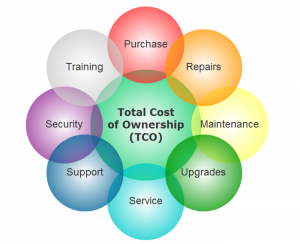
\includegraphics[width=0.3\textwidth]{img/tco}
\caption[Bestandteile der Total Cost of Ownership]{Quelle:
  \url{http://www.tritechamerica.com/total-cost-of-ownership/}, Stand:
  20.04.2016}
\end{figure}

Eine weitere Baustelle ist die mangelnde Datensicherheit und der
Datenschutz. Dies ist unter anderem zurückzuführen auf die unsichere
Anbindung der Franchise-Filialen, den Standort des Servers (im Keller
der Zentrale), das Accessmanagement für den Server-Zugriff (jeder
Mitarbeiter der Franchise-Filialen kann auf den Server und die
Unternehmensdaten zugreifen, da diese auf ein und demselben Server
liegen).

Ebenfalls wird deutlich, dass die Server-Architektur keinerlei
flexible Skalierbarkeit bietet, da Hardware bei Kapazitätserweiterung
erst bestellt und angeschafft werden muss. Diese neue Anschaffung und
vor allem die neue Einrichtung der Hardware kosten Zeit und
Geld. Somit ist eine flexible Skalierbarkeit unabkömmlich sobald die
Firma expandieren will beziehungsweise den Expansions-Gedanken schon
im Kopf hat.

Durch die vorhergehende Problemanalyse wird deutlich, dass vor allem
die Prozesse Optimierungspotential bieten und es muss ein interner
Standard im Bereich der Hard- und Software eingeführt werden.

Um nun die IT-Mitarbeiter zu entlasten und deren Überforderung zu
reduzieren muss zuerst eine Standardisierung der IT-Ausstattung (Hard-
und Software) vorgenommen werden. Dazu zählt, dass die verwendete
Hardware von nur einem Hersteller bezogen wird und sich die Modelle
nicht grundlegend unterscheiden. Ebenfalls muss die Software
lizenziert sein und aus einer sicheren und verlässlichen Quelle
stammen. Darüber hinaus werden so unter anderem die Wartungskosten und
der Wartungsaufwand gesenkt.

Als Lösung für die anderen Probleme, wie hoher Wartungsaufwand und
hohe Wartungskosten, mangelnder Datenschutz und Datensicherheit und
keine flexible Skalierbarkeit, bietet sich das Einführen einer Cloud
in das Unternehmensnetzwerk an. Genauer gesagt wird hier die Option
Infrastructure as a Service in Betracht gezogen und der im Keller
befindliche Server wird zu eigenen Datenbankserver auf dem die Kunden-
und Unternehmensdaten gespeichert sind.

Eine Cloud bietet mehrere Vorteile. Ein großer Vorteil ist, dass sich
eine Cloud flexibel skalieren lässt und sich so den verändernden
Unternehmensbedingungen anpassen kann. Wenn beispielsweise mehr
Speicherkapazität auf dem Cloud-Server benötigt wird, kann dies ohne
Probleme und schnell beim Cloud-Anbieter nachbestellt werden, es muss
keine zusätzliche Hardware bestellt und eingerichtet werden, da es
alles virtuell geschieht. In die andere Richtung ist die
Skalierbarkeit natürlich ebenfalls möglich. Es wird also nur das
bezahlt, was man auch wirklich braucht. Weitere Vorteile sind, dass
durch eine Cloud der Wartungs- und Upgrade-Aufwand gemindert wird, da
dies komplett der Cloud-Anbieter übernimmt. Ebenfalls wird so eine
sichere Plattform bereitgestellt und es kann über eine sichere
Verbindung mit der Cloud kommuniziert werden.

Auf dieser hybriden Cloud, das heißt, dass die Cloud sowohl aus einer
Public- (angeboten vom Cloud-Anbieter als \acrshort{IaaS}) als auch einer
Private-Cloud (eigener Server im Keller) besteht, werden nun die
benötigten Systeme (wie der Webshop oder andere IT-Systeme
(ServiceDesk, CRM, ERP und/oder Solution Manager)
bereitgestellt\footnote{Vgl.~ITwissen.info (o.J), Hybrid Cloud,
  Online im Internet}. Die Systeme in der Cloud erhalten ihre Daten
(Kunden-, Einkaufs- oder Unternehmensdaten) über eine sichere
Verbindung mit dem Datenbankserver, welcher sich in der Zentrale
befindet. So greift keiner der Franchise-Filialen mehr direkt auf die
sensiblen Daten zu, da sie nur direkt an die Cloud angebunden sind und
lediglich Lese-Rechte auf die sensiblen Daten haben. So werden
versehentliche Änderungen in den Datensätzen vermieden.

Neben den bereits genannten Problemlösungen müssen ebenfalls die
Prozesse an den neuen Standard angepasst, optimiert und überarbeitet
werden, um so letztendlich auch beispielsweise vereinbarte \acrshort{SLA}’s
einhalten zu können. Hierfür muss das Rad nicht neu erfunden werden,
sondern es kann sich an ITIL bedient werden. ITIL ist eine Sammlung
von vordefinierten und standardisierten Prozessen, Funktionen und
Rollen. Es bietet Best-Practice Vorschläge, welche an das Unternehmen
angepasst werden können bzw.~müssen und eignet sich somit perfekt für
ein Start-up. ITIL besteht aus fünf ,,Phasen'', welche den
Service-Lifecycle widerspiegeln: Service Strategy (Servicestrategie),
Service Design (Serviceentwurf), Service Transition
(Serviceüberführung), Service Operation (Servicebetrieb) und Continual
Service Improvement (kontinuierliche
Serviceverbesserung)\footnote{Vgl.~(o.A) (2016), ITIL-Prozesse, Online
  im Internet}. Beispiele für ITIL-Standards bzw. Best-Practice
Prozesse wären: das Business Relationship Management (Service
Strategy\footnote{Vgl.~(o.A) (2016), ITIL Service Strategy –
  Servicestrategie, Online im Internet}) das Service Level-, Risiko-,
Compliance-, Supplier – Management (Service Design\footnote{Vgl.~(o.A)
  (2016), ITIL Service Design, Online im Internet}) das Change-,
Release-, Configuration – Management (Service
Transition\footnote{Vgl.~(o.A) (2016), ITIL Service Transition –
  Serviceüberführung, Online im Internet}), der ServiceDesk
bzw. Incident-, Problem-, Access-, Event – Management (Service
Operation\footnote{Vgl.~(o.A) (2016), ITIL Service Operation –
  Servicebetrieb, Online im Internet}) und Service Reviews (Continual
Service Improvement\footnote{Vgl.~(o.A) (2016), ITIL CSI -
  Kontinuierliche Serviceverbesserung, Online im Internet}),

Die vordefinierten Standards in ITIL können flexibel an das
Unternehmen ,,Stylez'' angepasst werden und helfen somit die Prozesse
zu optimieren und zu strukturieren und ,,Stylez'' kann sich an
vordefinierte Standards und Best-Practices bedienen und diese nutzen.

Abschließend lässt sich sagen, dass mit den erwähnten
Änderungsmaßnahmen alle Problemfelder, welche analysiert wurden
abgedeckt und behoben werden können.

Um nun die Veränderungen durchzuführen, kann sich ,,Stylez'' an den
vordefinierten Standards in ITIL für das Change Management bedienen
und kann diese an seine Bedürfnisse anpassen.

%!TEX root = ../Thesis.tex
\section{Balanced Scorecard (Patrick Künzl)}
\subsection{Definition}
Die Balance Scorecard ist eines von vielen Instrumenten, um eine zielführende
Komposition der Unternehmensthemen \glqq Strategiefindung\grqq~und
\glqq Strategieumsetzung\grqq~zu erreichen. \glqq In ihrem Konzept werden die
traditionellen finanziellen Kennzahlen durch eine Kunden-, eine 
interne Prozess- und eine Lern- und Entwicklungsperspektive
ergänzt.\glqq\footnote{siehe \cite{BalanceGabler}} \\
Die Balance Scorecard wurde in den 90er-Jahren von R.S. Kaplan und D.P. Norton
entwickelt und war das Resultat einer Studie unter zwölf amerikanischen
Unternehmen. Ziel der Studie war es, die damalig vorhandenen Kennzahlensysteme
an den neuzeitigen Anforderungen der Unternehmen anzupassen. \footnote{Vgl.
\cite{BalanceGabler}}
\subsection{Aufbau der Balance Scorecard}
\begin{figure}[H]
\centering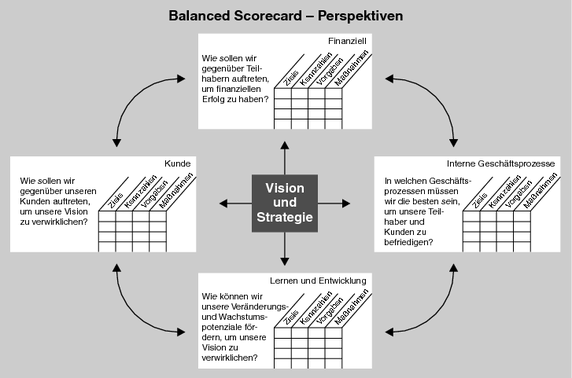
\includegraphics[width=1\textwidth]{img/bsc}
\caption[Aufbau einer Balance Scorecard]{schematische Darstellung des Aufbaus
einer Balance Scorecard - Quelle:
http://wirtschaftslexikon.gabler.de/Definition/balanced-scorecard.html,
Stand 03.04.2016}
\end{figure}
Die Balance Scorecard betrachtet das Unternehmen durch vier unterschiedliche
Perspektiven, welche nachfolgend kurz umschrieben werden:
\begin{itemize}
  \item finanzielle Sichtweise: \\
  Die finanzielle Sichtweise ist die älteste Perspektive des Modells. Dies kommt
  dadurch, dass die Basismodelle des Unternehmenscontrollings in den 50er Jahre
  die finanziellen Kennzahlen größtenteils als die einzig verlässlichen
  Parameter für den Erfolg eines Unternehmens lieferten. Die zentrale Frage, welche die
  finanzielle Perspektive beantworten möchte, lautet: \glqq Haben unsere getroffenen
  Maßnahmen und Strategien einen erfolgreichen Einfluss auf unseren
  Unternehmenserfolg?\glqq
  \item interne Geschäftsprozesse: \\
  Die Sicht der internen Geschäftsprozesse bietet die Möglichkeit Kennzahlen
  für, z. B. Durchlaufzeiten von verschiedenen Prozessen oder andere
  geschäftskritischen Workflows, zu analysieren und zu steuern. Ziel der Analyse
  der internen Prozesse beantwortet die Frage: \glqq In welchen Geschäftsprozessen
  müssen wir die besten sein, um unsere Teilhaber und Kunden zu befriedigen?\glqq
  \footnote{Vgl. mit obiger Abbildung}
  \item Lern- und Wachstumsperspektive: \\
  Die Lern- und Wachstumsperspektive ist die wichtigste Perspektive der gesamten
  Balanced Scorecard und bildet somit die Basis. Denn mit der Betrachtung der
  Mitarbeiter und den \glqq sozialen Faktoren\grqq~können erst alle anderen Ziele in 
  den anderen erreicht werden. \glqq Drei Hauptkategorien werden hierbei
  unterschieden: Qualifizierung von Mitarbeitern, Leistungsfähigkeit des 
  Informationssystems sowie Motivation und Zielausrichtung von Mitarbeitern.\glqq
  \footnote{siehe \cite{BalanceGabler}}
  \item Kundenperspektive: \\
  Die Kundenperspektive kümmert sich um jegliche Kennzahlen, die sich um den
  Kunden drehen. Es ist hierbei jedoch nicht zwingend notwendig, dass es externe
  Kunden sein müssen, sondern auch firmeninterne Abteilungen können Kunden für
  eine Abteilung sein, z. B. für die IT.
\end{itemize}
Wie man anhand der obigen Abbildung erkennen kann, stehen alle Perspektiven in
einer engen Beziehung zueinander, einer sogenannten
\glqq Ursache-Wirkung-Beziehung\glqq. Dies bedeutet, dass jegliche Anpassungen in einer
Perspektive ebenso Änderungen in anderen Perspektiven und den damit verbundenden
Kennzahlen mit sich bringt.
\subsection{Design der Balanced Scorecard für das Unternehmen Stylez}
Nachfolgend wird eine Strategie für das Unternehmen Stylez dargelegt. Dabei wird
jede Perspektive einzeln betrachtet und ausführlich dargestellt.
\subsubsection{finanzielle Perspektive}
\emph{Strategisches Ziel:} Um die eigene Marktposition weiter auszubauen, soll
die Anzahl der Franchise-Filialen weiterhin stark ansteigen\\
\emph{Kennzahl/Messgröße:} Anzahl der Franchise-Filialen\\
\emph{Zielwert:} 6 neue Filialen pro Jahr \\
\emph{Erforderliche Maßnahmen:} Durchführung einer guten Marketing-Strategie,
stetiger Ausbau des Bekanntheitsgrades, das Führen von Franchise-Filialen
attraktiver gestalten\\\\
\emph{Strategisches Ziel:} Erhöhung der Umsatzrendite im Online-Geschäft\\
\emph{Kennzahl/Messgröße:} Umsatzrendite des Online-Shops\\
\emph{Zielwert:} Steigerung um 3 Prozent \\
\emph{Erforderliche Maßnahmen:} Optimierung der IT-Infrastruktur, Verhandeln
von besseren Lieferantenkonditionen, Erhöhung der Gewinnspanne
\subsubsection{Kundenperspektive}
\emph{Strategisches Ziel:} Durch Anreizsysteme sollen Bestandskunden öfters
Neukunden werben\\
\emph{Kennzahl/Messgröße:} Neukunden pro Monat\\
\emph{Zielwert:} 25 Neukunden pro Monat \\
\emph{Erforderliche Maßnahmen:} Entwicklung eines Anreizsystems durch
Einführung eines Rabattsystems\\\\
\emph{Strategisches Ziel:} interne Abteilungen sollen zufriedener mit der
IT-Abteilung werden\\
\emph{Kennzahl/Messgröße:} Zufriedenheitsgrad der Mitarbeiter\\
\emph{Zielwert:} mindestens 4 von 5 Sternen \\
\emph{Erforderliche Maßnahmen:} Optimierung der IT-Infrastruktur, Mitarbeiter in
den Abteilungen schulen um kleinere Probleme selbst zu lösen, Einführung eines
Ticketsystem und Vorpriorisierung der Aufgaben für die IT-Mitarbeiter
\subsubsection{interne Prozessperspektive}
\emph{Strategisches Ziel:} benötigte Unternehmensdaten sollen den
Franchise-Filialen schneller zur Verfügung stehen\\
\emph{Kennzahl/Messgröße:} Geschwindigkeit der Datenabfrage und Transport in die
Filiale\\
\emph{Zielwert:} unter 5 Sekunden um jede Information zu bekommen \\
\emph{Erforderliche Maßnahmen:} Optimierung der Verbindungsleitungen,
Optimierung der IT-Infrastruktur, Fokus auf Hochverfügbarkeit von Daten
setzen\\\\
\emph{Strategisches Ziel:} Verkürzung der Wartungsarbeiten für IT-Mitarbeiter\\
\emph{Kennzahl/Messgröße:} Dauer der Wartungsarbeit\\
\emph{Zielwert:} pro Server im Haus nicht länger als 10 Minuten \\
\emph{Erforderliche Maßnahmen:} Optimierung der IT-Infrastruktur, Auslagerung
von Unternehmenssystemen nach Drittanbietern
\subsubsection{Lern- und Entwicklungsperspektive}
\emph{Strategisches Ziel:} Probleme bestehen in jeder Firma. Um die
Mitarbeiter an der Optimierung des Unternehmens teilhaben zu lassen, wird ein
betriebliches Verbesserungssystem eingeführt. Die Mitarbeiter sollen jedoch
selbst entscheiden, ob sie dran teilnehmen oder nicht.\\
\emph{Kennzahl/Messgröße:} Anzahl der Verbesserungsvorschläge pro Monat\\
\emph{Zielwert:} 3 pro Mitarbeiter pro Monat \\
\emph{Erforderliche Maßnahmen:} Einführung des betrieblichen
Vorschlagwesens, Einarbeitung der Mitarbeiter durch ein Anreizsystem bei
Durchführung\\\\
\emph{Strategisches Ziel:} konsequente Weiterbildung aller Mitarbeiter\\
\emph{Kennzahl/Messgröße:} Anzahl der Weiterbildungstage\\
\emph{Zielwert:} Mindestens 5 Tage pro Jahr \\
\emph{Erforderliche Maßnahmen:} Erweiterung des Schulungsangebots, Versand von
E-Mails mit externen Weiterbildungsmöglichkeiten, Einrichtung einer zentralen
Stelle zur Annahme von individuellen Weiterbildungsanfragen
\section{IT-Infrastruktur (Patrick Künzl)}
\label{sec:IT-Infrastruktur}
\subsection{Einleitende Worte}
Rückblickend auf die Balanced Scorecard erkennt man, dass viele Maßnahmen zur
Zielerreichung sich auf die Optimierung der IT-Infrastruktur stützen. Dies hat
in einem Unternehmen, welches sein Gewinn ausschließlich mit einem
Online-Geschäft und seiner Bereitstellung von Unternehmensdaten an nationale
Filialen erwirtschaftet, durchaus seine Berechtigung. Um diesen Gewinn nicht zu
gefährden, muss die IT-Strategie perfekt auf die Unternehmensstrategie angepasst
sein und muss die Anforderungen zur vollsten Zufriedenheit erfüllen.
Beispielhafte Anforderungen für die Zukunft wären:
\begin{itemize}
  \item Wahrung der Verfügbarkeit von Daten ohne Rücksicht auf Anzahl der
  eintreffenden Anfragen
  \item Wahrung eines optimalen Preis-/Leistungs-Verhältnisses
  \item Sicherung des Unternehmenserfolges
  \item Sicherung des Umsatzes
\end{itemize}
Die IT-Strategie versucht nun durch\ldots
\begin{itemize}
  \item \ldots eine leichte Skalierbarkeit der Hardware
  \item \ldots Verteilung der Auslastung und Abfangen von Belastungsspitzen
  \item \ldots Optimierung des Kostenspiegels
\end{itemize}
die Unternehmensstrategie erfolgreich zu unterstützen. Die Basis bildet dafür
die \glqq Grundhardware\glqq, die das Rückgrat der Unternehmens-IT bildet.
\subsection{Grundgedanke}
Start-Ups haben eine schwierige Ausgangssituation die interne IT zu optimieren.
Durch die fehlende Sicherung eines Wettbewerbsplatzes und der schwierigen
Abschätzbarkeit der notwendigen Ressourcen bei gleichzeitiger optimalen
Kostenkontrolle muss ein besonderes Augenmerk auf die Auslastung der Server
gelegt werden, da diese der Kostentreiber der IT sein können. Hier darf kein
Potenzial verschenkt werden. Daher wird der Vorschlag getätigt, die bisherigen
Server in der Unternehmenszentrale als Datenbankserver des Unternehmens
einzusetzen und Softwaresysteme mittels Infrastructure-as-a-Service
bereitzustellen, die wiederum per Direktleitung mit der Datenbank kommunizieren.
\subsubsection{Infrastructure-as-a-Service}
Bei Infrastructure-as-a-Service handelt sich um eins von vielen möglichen
Cloud-Modellen. Die Vorteile solch eines IT-Modells sind vielfältig: 
\begin{itemize}
  \item Kostenvorteile durch bedarfsgerechte Anpassung
  \item vorkonfektionierte Umgebungen mit modernster Technologie und sicherer
  Plattform
  \item keine Aufwände für Upgrades, Betrieb und Wartung
  \item Belastungsspitzen werden besser aufgefangen
  \item schnelle Skalierung des Systems auf die Echtzeit-Anforderungen
\end{itemize}
Datenschutzrichtlinien, Verbindungssicherheit und hohe Verfügbarkeit machen
Infrastructure-as-a-Service zu einem sehr attraktiven Gesamtpaket für junge
Unternehmen, die noch in der Aufbau- bzw. Expansionsphase sind. \\
Um dennoch weiterhin die Hoheitsrechte über die Unternehmensdaten zu wahren und
im extremsten Fall direkt und zu 100 Prozent über alle Daten zu verfügen, wird
die bisher bestehende Hardware in einen reinen Datenbankserver umgewandelt. Dieser
Datenbankserver gilt als zentrale Anlaufstelle für jegliche Software und ist per
direkter Leitung an die Cloud-Systeme der Anbieter angebunden, um eine schnelle
Übermittlung der Bytes zu gewährleisten.
\subsection{Amazon Web Services - Beispielrechnung}
\label{sec: AWS_Rechnung}
Um zu zeigen, dass es sich durchaus lohnt das IaaS-Konzept in die
Unternehmensstruktur aufzunehmen, anstatt die einzelnen Komponenten selbst zu
betreiben, betrachten wir die Gesamtkosten (Total Cost of Ownership) von einem
selbst-gekauften Server und einem angemieteten IaaS-Server.
\\ \\
\emph{Kostenaufstellung: eigener Server - Laufzeit 5 Jahre}
\begin{itemize}
  \item Anschaffungskosten:
  	\begin{itemize}
  	  \item Hardware: 2650\euro
  	  \item Betriebssystem (Server 2012 + CALs): 10000\euro
  	  \item Installationskosten: 1 MA, 8 Stunden für 110\euro/Stunde = 880\euro
  	\end{itemize}
  \item Betriebskosten:
  	\begin{itemize}
  	  \item Strom: 20\euro * 12 Monate * 5 Jahre = 1200\euro
  	  \item Wartung des Servers: 1 MA, 4 Stunden für 110\euro/Stunde, 1x pro
  	  Monat = 26400\euro
  	  \item Kosten für Ersatzteile: 1000\euro
  	\end{itemize}
  \item Entsorgungskosten:
  	\begin{itemize}
  	  \item Entsorgung: 100\euro
  	  \item Mitarbeiteraufwand: 1 MA, 4 Stunden für 110\euro/Stunde = 550\euro
  	\end{itemize}
  \item Gesamtsumme: 42780\euro
\end{itemize}
\underline{Kostenaufstellung: EC2 Server auf Amazon Web Services - Laufzeit 5
Jahre\footnote{die Preisangaben beziehen sich auf ein offizielles Whitepaper
von Amazon und sind dort in Dollar angegeben, Umrechnungskurs zum Euro: 1 US
Dollar = 0,87769\euro}}
\begin{itemize}
  \item Anschaffungskosten:
  	\begin{itemize}
  	  \item Hardware: 0\euro
  	  \item Betriebssystem (Server 2012 + CALs): 0\euro
  	  \item Installationskosten: 1 MA, 1 Stunde für 110\euro/Stunde = 110\euro
  	\end{itemize}
  \item Betriebskosten:
  	\begin{itemize}
  	  \item Strom: 20\euro * 12 Monate * 5 Jahre = 0\euro
  	  \item Wartung des Servers: 1 MA, 4 Stunden pro Jahr für 110\euro/Stunde =
  	  550\euro
  	  \item Kosten für Ersatzteile: 0\euro
  	  \item Amazon EC2 Instance Cost: Kosten pro Stunde 0,0614383\euro, 2
  	  Instanzen, 732 Stunden pro Monat = 5396,74\euro
  	  \item Elastic Load Balancer Cost: 732 Stunden pro Monat, Stundensatz von
  	  0,02194225\euro, Verarbeitete Daten [GB] 3000, Verarbeitungssatz von
  	  0,00702152\euro = 2227,58\euro
  	  \item AWS Data Transfer Cost: Empfangene Daten [GB] 2700 für 0,00\euro,
  	  Gesendete Daten [GB] 4100 für 0,1053228\euro = 25909,41\euro
  	\end{itemize}
  \item Entsorgungskosten:
  	\begin{itemize}
  	  \item Entsorgung: 0\euro
  	  \item Mitarbeiteraufwand: 1 MA, 1 Stunden für 110\euro/Stunde = 110\euro
  	\end{itemize}
  \item Gesamtsumme: 34303,73\euro
  \item Ersparnis gegenüber Self-Hosting-Variante: 8476,27\euro
\end{itemize}
Hier ist deutlich erkennbar, dass die Verwendung einer
Infrastructure-as-a-Service Lösung enorme Sparpotenziale hervorbringen kann.
Besonders durch die gesunkenen Aufwände für Wartung und die Verwendung dieser
gewonnenen Arbeitszeiten in andere Projekte, können die finanziellen
Strategieziele des Unternehmens optimal unterstützt werden.

%!TEX root = ../Thesis.tex
\section{Multichannel-System in der Cloud (An-Nam Pham)}
Das Unternehmen Stylez betreibt ein Multichannel-Retailing (Mehrgleisiger Vertrieb des Handels). Wie in der Grafik \ref{img:Cloud_Implementierung} auf Seite \pageref{img:Cloud_Implementierung} zu sehen, kann der Kunde sowohl in der Filiale, als auch online per Webshop einkaufen. Gekaufte Waren können bei Bedarf ebenfalls sowohl in einer Filiale als auch online umgetauscht oder zurückgegeben werden (beim Online-Weg: Rücksendung per Post).

Die Aufgabe diese Prozesse zu steuern und zu überwachen, ist ohne Unterstützung von passender IT-Systeme kaum zu bewältigen.\\
Die Lösung für die große Multichannel-Herausforderung lautet Multichannel-System.\\
\\
Das Multichannel-System ist ein Verbund von mehreren Systemen, die dem Unternehmen dabei unterstützen, sämtliche Geschäftsprozesse und das Kundenmangement zu steuern.\\
\\
Im Kapitel \ref{sec:IT-Infrastruktur} wurden die Vorteile für einen Umzug in die Cloud erläutert.
Deswegen soll das Multichannel-System in der Cloud betrieben werden.
Die zentrale Datenbank ist die Datenbasis für das Multichannel-System. Da hier nicht nur Unternehmensdaten, sondern auch vertrauliche Kundendaten gespeichert werden, soll diese Datenbank nicht in die Cloud ausgelagert werden, sondern weiterhin vom Unternehmen betrieben werden.

Dies macht das Ganze zu einer hybriden Cloud, die aus der Private Cloud (zentrale Datenbank) und der Public Cloud besteht.\\
\\
Die folgende Abbildung zeigt die empfohlene Implementierung des Multichannel-Systems in der Hybrid Cloud:
\begin{figure}[H]
\centering
\begin{minipage}[t]{0.8\textwidth}
\fbox{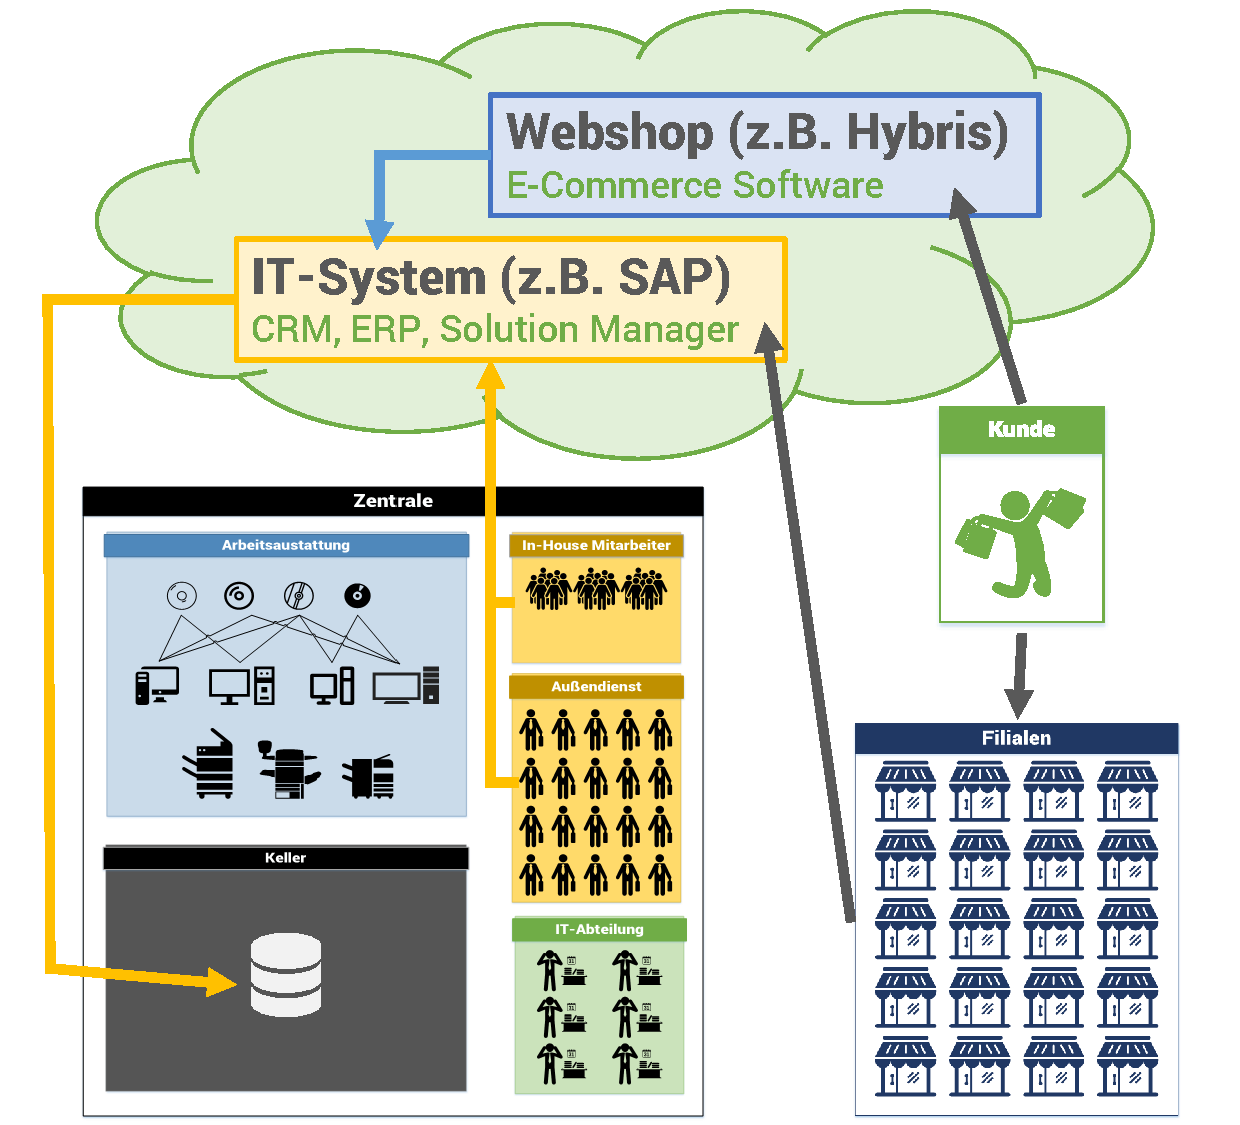
\includegraphics[width=1\textwidth]{img/Cloudinhalt.pdf}}
\caption{Empfohlene Implementierung der Hybrid Cloud} % Überschrift
\source{Eigene Darstellung} % Quelle
\label{img:Cloud_Implementierung}
\end{minipage}
\end{figure}
In den folgenden Unterkapiteln werden die einzelnen Komponenten des Multichannel-Systems kurz beschrieben und ihr Nutzen für das Unternehmen erläutert.
\subsection{SAP IT-System}
Wir empfehlen die gesamte Unternehmensstruktur von Stylez mit Hilfe von SAP im IT-System abzubilden\footnote{Berechtigungskonzept, Organisationsmanagement, Geschäftsprozesse, etc. werden in SAP ERP abgebildet, um ein optimales Business-IT-Alignment zu ermöglichen.}. Der Entscheidung für SAP bietet unter anderem folgende Vorteile\footcite{SAP_Vorteil}:
\begin{itemize}
\item Internationaler Anbieter
\item führende Technologie
\item 40 Jahre Erfahrung mit kfm. Software
\item technische Innovationskraft
\item finanzielle Stabilität
\end{itemize}
Außerdem gibt es viele SAP-Partner, die auf den Fashion-Handel spezialisiert sind. Diese haben unter anderem folgende Stärken:
\begin{itemize}
\item Kundennähe
\item Mittelstandsausrichtung und -erfahrung
\item Angebot als Generalunternehmer
\end{itemize}
Das SAP System soll aus ein \acrshort{ERP}-System, \acrshort{CRM}-System und einen Solution Manager bestehen.
\subsubsection{SAP ERP}
Das \acrlong{ERP}-System (ERP-System) bildet (im Idealfall) das Unternehmen in seiner Gesamtheit zeitnah ab. Dadurch ist es ein sehr wertvolles Hilfsmittel für Planungs- und Steuerungsaufgaben, das unter anderem noch folgende Vorteile bietet:
\begin{itemize}
\item Erhöhte Automatisierung für kürzere Bearbeitungszeiten und Kostenersparnisse
\item Verringerte Durchlaufzeiten von Prozessen
\item Erhöhte Datenqualität, Redundanzen und Inkonsistenzen werden vermieden
\item Verbesserte Zusammenarbeit über Abteilungsgrenzen hinweg
\item Optimierter Informationsfluss im Unternehmen
\item Überwinden organisatorischer und technischer Schnittstellen
\end{itemize}
\underline{\textbf{Der große Nutzen:}}\\
ERP-Systeme tragen langfristig zur Leistungssteigerung und Kostenreduzierung bei, da das ERP-System sämtliche Bereiche wie z.B. Materialwirtschaft, Finanz- und Rechnungswesen, Personalwirtschaft, Verkauf, Marketing und Forschung abbildet. Dadurch können alle Bereiche miteinander kommunizieren und dieselbe Datenbasis nutzen. Dies spart z.B. im Vergleich zur \glqq Zettelwirtschaft\grqq~und Excel viel Zeit und Kosten.\footcite[vgl.][]{ERP}
\subsubsection{SAP CRM}
\glqq Der Kunde ist König\grqq. Dieser bekannte Satz drückt ganz gut aus, worauf man in einem Unternehmen ganz besonders achten muss.\\
Das \acrlong{CRM} (CRM) (zu Deutsch: Kundenbeziehungsmanagement) unterstützt das Unternehmen dabei, die Beziehung zu bestehenden und potenziellen Kunden zu verwalten und zu gestalten.\\
\\
\underline{\textbf{Der große Nutzen:}}\\
Das CRM-System verwaltet nicht nur bestehende und potenzielle Kunden des Unternehmens. Wird das Supply-Chain-Management eingebunden, kann das CRM-System auch Lieferanten verwalten. Im Fall von Stylez können auch alle Franchisenehmer eingebunden werden.\\
Das Besondere am CRM-System ist, dass es die Historie der Kundeninteraktion verfolgbar macht. Es kann sehr schnell ein Überblick über einen Kunden, Lieferanten oder Franchisenehmer\footnote{Zur Vereinfachung werden Kunden, Lieferanten oder Franchisenehmer im Folgenden mit Kunde zusammengefasst.} geschaffen werden (z.B. getätigte Anrufe, Häufigkeit der Support-Anfragen, Anteil am Geschäftsumsatz, uvm.).
Dadurch kann schnell auf den Kunden eingegangen. Dies spart Zeit und fördert die Professionalität und somit auch das Vertrauen der Kunden. Außerdem kann das CRM-Systen benutzt werden, um Prognosen über zu erwartende Ergebnisse einfacher und genauer zu erstellen. Und es bietet volle Transparenz und bei Bedarf jederzeit Zugriff auf Kundeninformationen.\footcite[vgl.][]{CRM}

\subsubsection{SAP Solution Manager}
Der Solution Manager wird für SAP-Kunden kostenfrei mitgeliefert und vereinfacht die Implementierung, den Betrieb, die Überwachung und die Unterstützung von SAP-Produkte im Unternehmen. Dabei bildet der Solution Manager alle IT-Prozesse ab und erfüllt bei der Betreibung dieser Prozesse alle ITIL-Prozesse\footcite[vgl.][]{SAPITIL}.

Folgende Komponenten umfasst der Solution Manager:
\begin{itemize}
\item Implementierung und Upgrade
\item Change Control Management
\item Testunterstützung
\item IT- und Anwendungs-Support
\item Diagnose und Ursachenanalyse
\item Systemüberwachung mit Solution Monitoring
\item Service-Level-Management und Reporting
\item Service-Verarbeitung
\item Administration
\end{itemize}
\underline{\textbf{Der große Nutzen:}}\\
Mit Hilfe des Solution Managers kann die IT-Abteilung der Firma stark entlastet werden. Sämtliche IT-Prozesse wie z.B. der IT- und Answendungs-Support per Helpdesk oder auch die Systemüberwachung und Administration werden vom Solution Manager nach ITIL unterstützt. Dank Solution Manager wird viel Aufwand und Zeit für IT-Aufgaben im Unternehmen eingespart.\footcite[vgl.][]{SolutionManager}

\subsection{Hybris (Webshop)}
Hybris ist ein E-Commerce-, Marketing- und Billing-Produkt\footnote{Abrechnungs-Produkt} vom gleichnamigen Hersteller, das seit 2013 zu SAP gehört\footcite[vgl.][]{SAPHybris}. Hybris wird für das Unternehmen Stylez empfohlen, da es:
\begin{enumerate}
\item auf Multichannel spezialisiert ist,
\item voll kompatibel mit SAP-Systemen ist,
\item Kundendaten in Echtzeit auswerten kann und
\item flexibel skalierbar ist.
\end{enumerate}
Außerdem wird Hybris vom unabhängigen Analysten Gartner als führend im Bereich Digital-Commerce-Software eingestuft\footcite{Gartner}.

\underline{\textbf{Der große Nutzen:}}\\
Als Komplettlösung für moderne Commerce Anwendungen, bietet Hybris dem Unternehmen einen leistungsstarken Webshop, das skalierbar und genau auf die Anforderungen von Stylez angepasst werden kann.

Herkömmliche Marketingkampagnen schaffen es nicht, individuelle Kunden anzusprechen. Deswegen werden stattdessen Massenbotschaften ohne individuelle Ansprache verbreitet

Hybris hilft dem Unternehmen in Verbindung mit SAP CRM anhand von Echtzeit-Kundenauswertungen dabei, den Kunden besser zu verstehen: was sie getan haben, was sie tun werden und, was am wichtigsten ist, was sie gerade tun. Dadurch kann der Kunde besser (z.B. durch Vorschläge im Shop oder angepasste Werbung) angesprochen werden.

Auch in einer Filiale kann der Kunde besser beraten werden, da sein bisheriges Einkaufsverhalten ein Echtzeit analysiert werden kann.

Wird Hybris auf das SAP IT-System aufgesetzt, sorgt es also für ein ansprechendes Einkaufserlebnis des Kunden und eine leichtere Verwaltung und Steuerung der Marketing- und Vertriebsprozesse.\footcite[vgl.][]{Hybris}
\section{So funktioniert der Umzug in die Hybrid Cloud (An-Nam Pham)}
% \section{Stichwort: Hochverfügbarkeit}
%\section SAP Rapid Deployment Solution
\section{Roadmap (An-Nam Pham)}

\section{Weitere IT-Maßnahmen (Vasilij Schneidermann)}

In der Analyse wurden zusätzlich zu der großen Baustelle Cloud noch
drei weitere Verbesserungspotenziale identifiziert: Die uneinheitliche
Arbeitsplatzausstattung, der überforderte IT-Support und die
Optimierung der Geschäftsprozesse.  Nahezu alle dieser Bereiche werden
durch den \emph{SAP Solution Manager} gelöst, jedoch ist es teilweise
möglich andere Lösungen für eine bessere Abdeckung hinzuzuziehen.  Zu
diesen gehören das \emph{SAP IT Infrastructure Management} und
\emph{Service Desk}.

\subsection{Arbeitsplatzausstattung}

Ehe eine einheitliche Arbeitsplatzausstattung verwendet werden kann,
ist es notwendig sich auf einen, oder besser, zwei IT-Ausstatter
festzulegen welche die nötige Infrastruktur zur Anbindung der
Cloud-Services bereitstellen können.  Gründe für mehr als einen
Ausstatter sind:

\begin{itemize}
\item Mehr Freiheit bei der Auswahl, da wenige Anbieter alle nötigen
  Bereiche gut bedienen können
\item Mehr Unabhängigkeit falls ein Anbieter nicht mehr die
  gewünschten Leistungen erbringen kann
\item Eine bessere Absicherung gegen Ausnutzung einer Einzelstellung
  des Anbieters
\end{itemize}

Eine denkbare Kombination wäre z.B.~Lenovo für Business-Laptops und
Dell für die verbleibende Peripherie (Monitore, Tastaturen, Mäuse,
etc.).  Je nach örtlicher Verfügbarkeit und Konditionen können
beliebige andere Anbieter ausgesucht werden.

Nach Vereinbarung eines Kooperationsvertrages kann mit einem
schrittweisen Rollout der neuen Hardware begonnen werden.  Zwar wäre
es auch möglich die Infrastruktur auf einen Schlag zu ersetzen, jedoch
ist dies generell nicht zu empfehlen, da etwaige Probleme beim Wechsel
sich über die gesamte IT-Landschaft erstrecken würden und in diesem
Falle es zu einem Totalausfall der IT kommen kann.  Im Gegensatz dazu
ist die kontinuierliche Ersetzung der alten Hardware weniger riskant,
verteilt die eingesetzten Kosten gleichmäßig über die Zeitdauer des
Rollouts und erlaubt es über den Vorgang hinweg wertvolles Feedback
der Mitarbeiter zu sammeln und umzusetzen.

An dieser Stelle ist es sinnvoll festzuhalten welche Hardware wo
eingesetzt wird.  Zu diesem Zweck kann der \emph{SAP Solution Manager}
durch das \emph{SAP IT Infrastructure
  Management}\footnote{Vgl.~\cite{SAP-IT-Realtech}, Online im
  Internet} erweitert werden, direkt nach Verkabelung der Geräte
werden ihre Seriennummern festgehalten und in die
CMDB\footnote{Configuration Management Database} eingetragen werden.
Neue Software wird von nun an nur noch aus autorisierten Quellen nach
Anfrage aufgespielt, so wird die Lizenzproblematik gekonnt umschifft.

Von diesem Zeitpunkt an ist die Hardware Teil des ERP-Prozesses: Der
Erwerb wird ordnungsgemäß festgehalten, ausgefallene Hardware kann
angefordert und nachbestellt werden, sie ist Teil des Inventars, die
dafür notwendige Software kann mit Leichtigkeit angefordert und
lizensiert werden, mithilfe von Monitoring und Berichten ist der
Infrastrukturstatus dem höheren Management stets bekannt, etc.  Da
jetzt auch der \emph{SAP Solution Manager} über das Inventar
informiert ist, kann man die Infrastruktur nun wie jeden anderen Teil
des Unternehmens verwalten und auftretende Probleme schnell
lösen\footnote{Vgl.~\cite{SAP-IT-Infrastructure-Management}, Online im
  Internet}.

\subsection{IT-Support}

Für die Bereitstellung eines idealen IT-Supports ist es notwendig
genau einen zentralen Zugriffspunkt zu haben.  Dieser muss nicht auf
ein Kommunikationsmedium zum Einreichen der sogenannten
\emph{Incidents} beschränkt sein, denkbar ist z.B.~eine Kombination
aus Benachrichtigung vom Produkt, bzw.~Anwendung heraus sowie einem
klassischen per Telefon und E-Mail erreichbaren \emph{Service
  Desk}\footnote{Vgl.~\cite{SAP-Service-Desk}, Online im Internet}.
Diese erhalten/erfassen für jeden Incident eine einheitlich gestaltete
Problembeschreibung, Priorität sowie weitere systemrelevante Daten wie
die Version der eingesetzten Software und das Betriebssystem des Kunden.

Zu diesem Zeitpunkt kann die Supportanfrage von einem automatisierten
System auf Merkmale wie den Supportlevel und einen ggf.~schon
vorhandenen Servicevertrag analysiert werden.  Sind diese bekannt,
weist das System die Anfrage einem Mitarbeiter zu, benachrichtigt
diesen und leitet sie bei Bedarf (wie z.B.~nach einer manuellen
Zuweisung an einen anderen Mitarbeiter) weiter.  Bei Bedarf können
noch fehlende Informationen wie E-Mail-Adresse und Telefonnummer vom
Kunden angefragt werden.

Die so vervollständigte Supportanfrage wird auf eine mögliche Lösung
untersucht.  Da ein Großteil auftretender Probleme dem Support schon
bekannt und wiederkehrender Natur ist, werden die beschriebenen
Symptome in einer sogenannten \emph{Customer Solution Database}
gesucht welche mit der Zeit durch neue Anfragen erweitert und bekannte
Anfragen verbessert wird.  Findet man eine möglicherweise anwendbare
Lösung, geht es an die Umsetzung seitens des Kunden, ansonsten wird
die Anfrage an ein höheres Supportlevel delegiert.  SAP bietet dafür
ein \emph{Support Back Office} an in welchem man sich nach Anforderung
der dafür nötigen Credentials mit ihnen austauschen kann.  Die so
erhaltene Lösung wird ähnlich der Lösungsdatenbank bereitgestellt,
sodass man auf den gleichen Workflow wie bei der internen
Lösungsfindung kommt.

Als nächstes kontaktiert man den Kunden mit der gefundenen Lösung und
hilft diesem sie anzuwenden und den Erfolg festzustellen.  Ist diese
erfolgreich, hinterlegt man sie in der \emph{Customer Solution
  Database}, andernfalls iteriert man durch andere gefundene Lösungen.
Schlussendlich markiert man das Supportticket als gelöst und bittet um
Kundenfeedback.  Dieses ist extremst wichtig um den IT-Support wirksam
zu steuern und den Kunden anzupassen.  Nur so kann sichergestellt
werden, dass dieser wirkungsvoll bleibt und den Ansprüchen der Kunden
gerecht wird.

Zur Integration in das Reporting werden in dieser IT-Support-Lösung
die Ticketzahlen nach Zeit/Abteilung, die Dauer der Bearbeitung,
Kundenzufriedenheit und interessante Verteilungen protokolliert.  Zu
diesen gehören:

\begin{itemize}
\item Über die \emph{Customer Solution Database} gelöste Tickets
\item Mit externen Hilfe gelösten Tickets
\item Menge an Tickets pro Abteilung
\item Tickets mit Konsequenzen im Change Management
\end{itemize}

Eine weitere wichtige Berücksichtigung ist, dass ein bestimmter Anteil
an Supportanfragen nicht immer nur durch interne und
SAP-Beratungsstellen gelöst werden kann, sondern es bei Bedarf auch
externe Help Desks geben kann welche z.B.~durch Outsourcing oder
anderweitig spezialisierte Expertise dafür besser geeignet sind.  Das
Service Desk kann auch bei Einbindung dieser externen Ressourcen
weiterhin deren Effizienz und Effektivität festhalten und diese somit
ähnlich wie die anderen Beratungsstellen integrieren kann.

\subsection{Kennzahlen und Benchmarking}

Ein an das Unternehmen angepasstes SAP-ERP-System erfasst
verschiedenste Daten, jedoch ist es notwendig die für die Zielsetzung
und -anpassung wichtigen Kriterien gesondert zu beobachten um anhand
der Soll- und Ist-Ergebnisse die Geschäftsprozesse anpassen zu
können.  Die so gewählten Kennzahlen dürfen dabei nicht in Isolation,
sondern müssen stets im Zusammenhang mit einer Zielgröße betrachtet
werden, erst dann ist ein Benchmarking durch einen Vergleich mit einem
anderen Report, einem anderen Unternehmens oder einer anderen Branche
möglich.

SAP schlägt für IT-Unternehmen vor die Bereiche \emph{Continuity},
\emph{Efficiency} und \emph{Compliance} zu
betrachten\footnote{Vgl.~\cite{SAP-Standard-IT-Service-Agreement},
  Online im Internet}.  Für die folgende Auflistung wurden für
sinnvoll erachtete Kennzahlen aus ihren Dokumenten sowie selbst
auserwählte mit typischen Zielgrößen genommen.

\begin{itemize}
\item Continuity
  \begin{itemize}
  \item Durchschnittliche Zeit zur Erstellung einer Supportanfrage (< 30min)
  \item Durchschnittliche Zeit für administrative Aufgabe (< 15min)
  \item Prozentualer Anteil durch das Help Desk gelöster Anfragen (> 90\%)
  \item Häufigkeit der Aktualisierung der Support Database (> 2x täglich)
  \item Durchschnittliche Uptime von IT-Services (> 99,9\%)
  \end{itemize}
\item Efficiency
  \begin{itemize}
  \item Kundenzufriedenheit (> 90\%)
  \item Dauer zur Bearbeitung interner E-Mails (< 1/2 Tag)
  \item Durchschnittliche Zeit zur Bearbeitung einer IT-Anfrage (< 1 Tag)
  \item Prozentualer Anteil durch 1st Level Support gelöster Anfragen (> 80\%)
  \item Prozentualer Anteil durch 2nd Level Support gelöster Anfragen (< 20\%)
  \item Anzahl insgesamt gelöster Anfragen (< 5/Tag)
  \item Maximale Ausfalldauer von IT-Services (< 1h)
  \item Durchschnittliche Response Time von IT-Services (< 1s)
  \end{itemize}
\item Compliance
  \begin{itemize}
  \item Interner Zufriedenheitsfaktor (> 80\%)
  \item Häufigkeit von SLA-Reviews (1/Periode)
  \item Ersparnisse durch umgesetzte Maßnahmen (> 20\%)
  \end{itemize}
\end{itemize}

Für die Auswertung der Kennzahlen ist der CTO zuständig.  Seine
Aufgabe ist es ein Auge auf der Entwicklung im Vergleich zu vorigen
Perioden zu behalten, eingeschränkte Prognosen zu machen und Berichte
sowie Änderungsmaßnahmen mit dem Rest der Führungsetage zu teilen.
Als Ergänzung zu klassischen Reports sind Dashboards denkbar.  Der
dafür nötige Prozess kann also in die folgenden Schritte unterteilt
werden:

\begin{enumerate}
\item Planung der Ziele und Maßnahmen
\item Umsetzung dieser in die Praxis
\item Testen der Implementierung mit Analyse der Ergebnisse
\item Anpassung der Maßnahmen und/oder Ziele
\end{enumerate}

Sollte seine Analysen ergeben, dass die Resultate die selbstgesteckten Ziele
stark verfehlen, wird er nach Best Practices Ausschau halten und diese
wo es Sinn ergibt umsetzen.

%!TEX root = ../Thesis.tex
\section{Fazit (An-Nam Pham)}

%!TEX root = ../Thesis.tex

% %%%%%%%%%%%%%%%%%%%%%%%%%%%%%%%%%%%%%%%%%%%%%%%%%%%%%%%%%%%%%%%%%%%%%%%
 %!TEX root = ../Thesis.tex
\section*{Quellenverzeichnis}
\addcontentsline{toc}{section}{Quellenverzeichnis}
\fancyhead[R]{Quellenverzeichnis}

\defbibheading{mono}{\subsection*{Monographien}}
\defbibheading{mag}{\subsection*{Aufsätze in Sammelbänden und Zeitschriften}}
\defbibheading{art}{\subsection*{Zeitungsartikel}}
\defbibheading{web}{\subsection*{Internetquellen}}
\defbibheading{leg}{\subsection*{Rechtsprechung}}
\defbibheading{comp}{\subsection*{Unternehmensunterlagen/Gesprächsnotizen}}
\defbibheading{webinar}{\subsection*{Webinare und Seminarunterlagen}}
\defbibheading{sap}{\subsection*{SAP Hilfe}}
\defbibheading{manus}{\subsection*{Firmeninterne Manuskripte}}
\defbibheading{interview}{\subsection*{Gesprächszusammenfassungen}}

\setlength\bibitemsep{1.5\itemsep}
\setlength{\bibhang}{2em}

\renewcommand{\baselinestretch}{1.50}\normalsize

\begingroup
\sloppy

% \printbibliography[keyword={mono},heading=mono]
% \printbibliography[keyword={sap},heading=sap]
% \printbibliography[keyword={mag},heading=mag]
\printbibliography[heading=web,keyword={web}]
% \printbibliography[heading=webinar,keyword={webinar}]
% \printbibliography[heading=manus,keyword={manus}]
% \printbibliography[heading=interview,keyword={interview}]
% Bei Bedarf einkommentieren: (erzeugt sonst Warnungen)
% \printbibliography[heading=art,keyword=art]
% \printbibliography[heading=leg,keyword=leg]
% \printbibliography[heading=comp,keyword=comp]

\endgroup
 %!TEX root = ../Thesis.tex

\section*{Ehrenwörtliche Erklärung}
\addcontentsline{toc}{section}{Ehrenwörtliche Erklärung}
\fancyhead[R]{Ehrenwörtliche Erklärung}

% Hiermit erkläre ich, dass ich die vorliegende \dokumententyp{} selbständig angefertigt habe. Es wurden nur die in der Arbeit ausdrücklich benannten Quellen und Hilfsmittel benutzt. Wörtlich oder sinngemäß übernommenes Gedankengut habe ich als solches kenntlich gemacht. Diese Arbeit hat in gleicher oder ähnlicher Form noch keiner Prüfungsbehörde vorgelegen.
% \vspace{20mm}

Hiermit erkläre ich, dass ich die mit meinem Namen gekennzeichneten Kapitel in der vorliegenden schriftlichen Ausarbeitung selbständig angefertigt habe. Es wurden nur die in der Arbeit ausdrücklich benannten Quellen und Hilfsmittel benutzt. Wörtlich oder sinngemäß übernommenes Gedankengut habe ich als solches kenntlich gemacht. Diese Arbeit hat in gleicher oder ähnlicher Form noch keiner Prüfungsbehörde vorgelegen.
\vspace{20mm}

\ort, \abgabedatum
\vspace{10mm}

\underline{\hspace{8cm}}\\Patrick Künzl
 
%%%%%%%%%%%%%%%%%%%%%%%%%%%%%%%%%%%%%%%%%%%%%%%%%%%%%%%%%%%%%%%%%%%%%%%

\end{document}